\section{Reflection on the product and process from a software engineering perspective}

In this section we will reflect on the software engineering part of our product and process. This means we will focus more on the code and development process rather than the result visible by the end-user. We will discuss the product and process in their own sections.

\subsection{Product}
When looking at our final product from a software engineering perspective, this means code-quality wise, we have managed to get a pretty decent result. We have tried to conform to coding standards by using Checkstyle\footnote{\url{checkstyle.sourceforge.net}} (for which we kept the error count at 0 on the stable branch at all times) and tried to find possible code smells by using PMD\footnote{\url{pmd.github.io}} and FindBugs\footnote{\url{findbugs.sourceforge.net}}.\\
We have implemented the MVC\footnote{\url{https://en.wikipedia.org/wiki/Model\%E2\%80\%93view\%E2\%80\%93controller}} design pattern in our code, and we kept the different components seperated very well. We have a single ControllerManager class that is linked with the model component. Next to this, there are all kinds of different controllers for different parts of the application. These can communicate with the ControllerManager and their own corresponding views that they control. All the logic happens in the controllers and the view classes purely focus on styling.\\
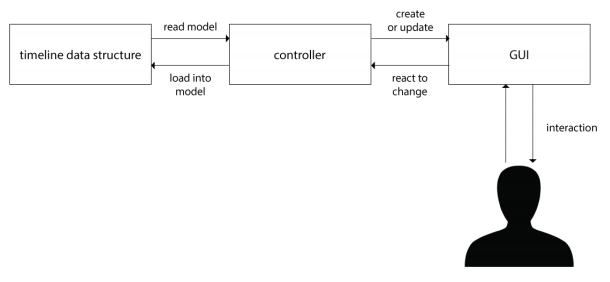
\includegraphics[scale=1]{./images/mvc}\\
\textit{Figure 1: Overview of the MVC pattern in our scripting application}\\\\
In our web application, we have used a RESTful architecture. This means that the server works with standard HTTP methods such as GET and POST, and that it doesn't store client session data. The session data is stored in a client's browser and, per request, the necessary session data is sent to the server in order to succesfully complete the request.\\
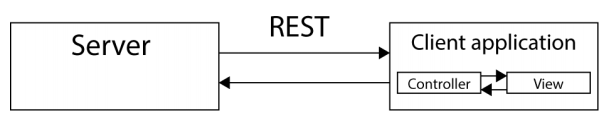
\includegraphics[scale=1]{./images/rest}\\
\textit{Figure 2: Server architecture}\\\\
A negative point lies in the fact that after a couple of weeks we found that the bugs got harder and harder to solve. It was clear that the maintainability of our system had gotten quite low. When looking back now, this was primarily during the fact that everyone was very eager to write code, and therefore did so, but there was just not enough communication about the exact design details. This led to some duplications and code that was hard to understand sometimes.\\
This point was was also found by the first SIG\footnote{\url{https://www.sig.eu/en}} evaluation, in which we got 6/10 ticks. After this, we worked hard to improve maintainability and it has definitely improved. We now have 8/10 ticks when running the same SIG evaluation again. Especially the amount of code duplication was reduced heavily.\\


\subsection{Process}
In this project we used SCRUM\footnote{\url{scrummethodology.com}}, an iterative and incremental agile software development framework for managing product development. This means that we worked in one-week sprints. At the beginning of a sprint we created a backlog/sprint plan, in which we wrote down user stories and the features that go with them. These features were to be implemented in that sprint. We also used prioritization to prioritize very important tasks, and give a low priority to tasks that did not need urgent completion. After each sprint we created a sprint retrospective, in which we reflected on the tasks we actually performed, and if there were any problems during the sprint.\\
When looking back at our SCRUM process, we have to say that we did not always exactly follow the sprint plan. Especially the division of who would do what was mostly thrown away. However, this did not cause much trouble because even though the sprint plan was not exactly followed, the general direction of features was still implemented. It's just that everyone worked on what they liked most rather than exactly follow the sprint plan. It did happen a few times that some high-priority items were not implemented, because everyone was working on something else and we forgot to keep the sprint plan in mind.\\
For communication we used Slack\footnote{\url{https://slack.com/}}. Also, next to communicating remotely, we found it important to try and work together in one place as often as possible. This is why we sat together almost every morning. Not only did this force us to work on the project instead of lying in bed, but the communication during these hours was very easy, and we could easily help each other out if someone was having problems. Overall, communication went very well, we almost always knew who was working on what.
